\chapter{Supplementary figures}
\label{app:figures}

% 3 - LOCUS CHAPTER

\begin{figure}
	\centering
	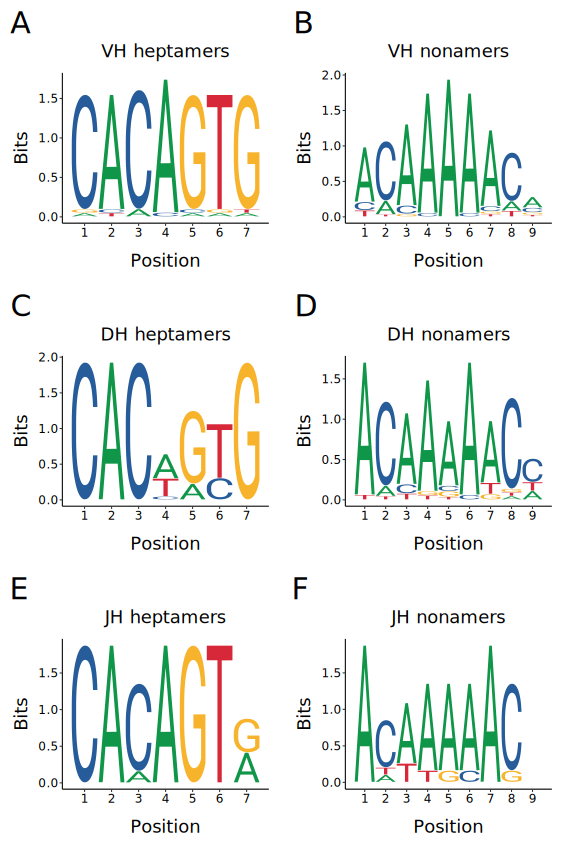
\includegraphics[width=0.9\textwidth]{_Figures/png/nfu-rss-seqlogo-sep}
	\caption[\Nfu recombination signal sequences by segment type]{\textbf{\Nfu recombination signal sequences by segment type:} Sequence composition of conserved heptamer (A,C,E) and nonamer (B,D,F) sequences from \Nfu heavy-chain RSSs associated with \vh (A,B), \dh (C,D) or \jh (E,F) gene segments.}
	\label{fig:nfu-rss-seqlogo-sep}
\end{figure}

\begin{figure}
	\centering
	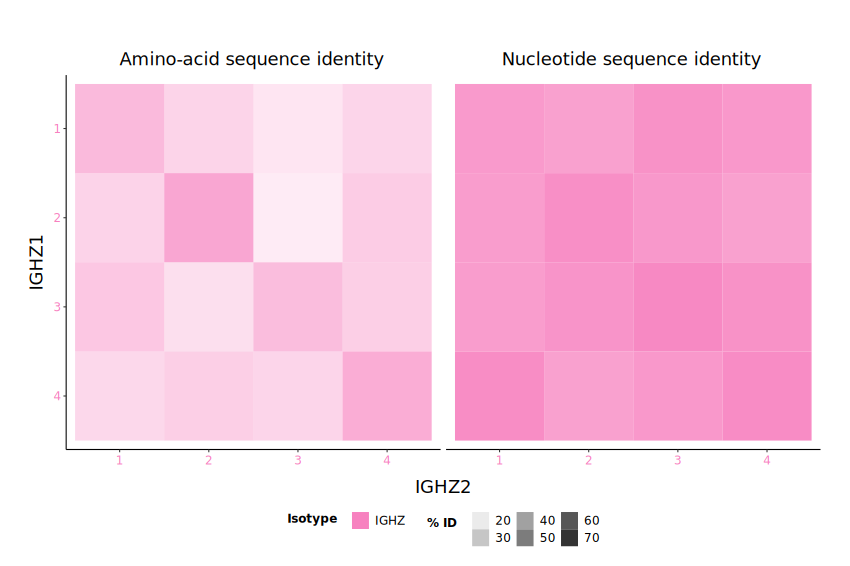
\includegraphics[width=0.8\textwidth]{_Figures/png/xma-new-cz-aln}
	\caption[Sequence similarity between \igh{Z} constant-regions in \Xma]{\textbf{Sequence similarity between \igh{Z} constant-regions in \Xma:} Heatmap of percentage sequence identity between amino-acid (right) and nucleotide (left) sequences of \cz{} exons from the two \Xma \igh{Z} constant regions, calculated using pairwise Needleman-Wunsch global alignments.} % TODO: Combine isotype and identity legends
	\label{fig:xma-cz-aln}
\end{figure}

	\begin{figure}
	\centering
	\includegraphics[width=\textwidth]{_Figures/png/xma-vh-families-map}
	\caption[Heatmap of \vh families in the in \Xma \textit{IgH} locus]{\textbf{Heatmap of \vh families in the in \Xma (\textit{IgH}) locus:} Heatmap of family relationships among \Xma \vh segments, with coloured shading indicating families and red dots indicating pairwise nucleotide sequence identity of at least 80\%. \vh families containing multiple segments are uniquely coloured, while single-segment families are in grey.}
	\label{fig:xma-vh-families-map}
	\end{figure}

	\begin{figure}
	\centering
	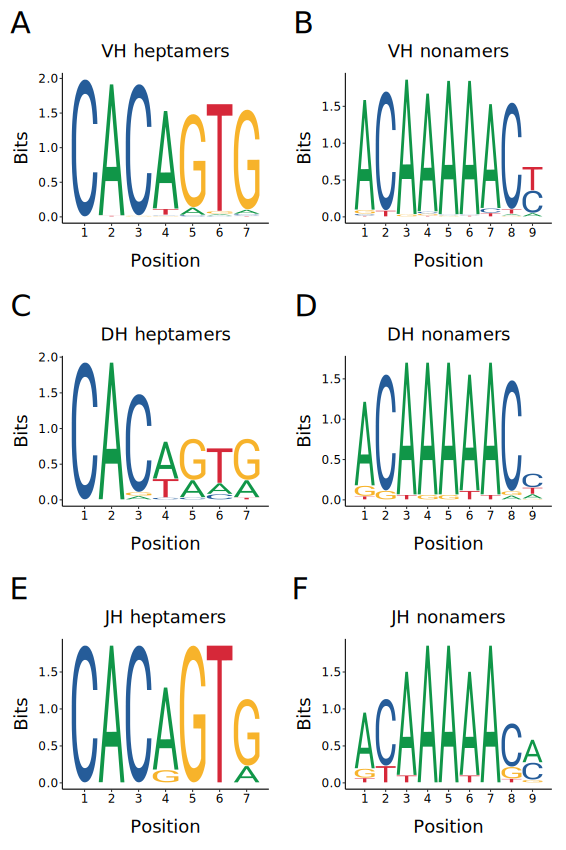
\includegraphics[width=0.9\textwidth]{_Figures/png/xma-new-rss-seqlogo-sep}
	\caption[\Xma recombination signal sequences by segment type]{\textbf{\Xma recombination signal sequences by segment type:} Sequence composition of conserved heptamer (A,C,E) and nonamer (B,D,F) sequences from \Xma heavy-chain RSSs associated with \vh (A,B), \dh (C,D) or \jh (E,F) gene segments.}
	\label{fig:xma-rss-seqlogo-sep}
	\end{figure}